%%%%%%%%%%%%%%%%%%%%%%%%%%%%%%%%%%%%%%%%%%%%%%%%%%%%%%%%%%%%%%%%%%%%%%%%%%%%%%%%
% Front matter
%%%%%%%%%%%%%%%%%%%%%%%%%%%%%%%%%%%%%%%%%%%%%%%%%%%%%%%%%%%%%%%%%%%%%%%%%%%%%%%%

\title{pdp: An R Package for Constructing Partial Dependence Plots}
\author{by Brandon M. Greenwell}

\maketitle

\abstract{
Complex nonparametric models---like neural networks, random forests, and support vector machines---are more common than ever in predictive analytics, especially when dealing with large observational databases that don't adhere to the strict assumptions imposed by traditional statistical techniques (e.g., multiple linear regression which assumes $E\left[\boldsymbol{\mathcal{Y}}\right] = \boldsymbol{X}\boldsymbol{\beta}$). Unfortunately, it can be challenging to understand the results of such models and explain them to management. Partial dependence plots offer a simple solution. Partial dependence plots are low-dimensional graphical renderings of the prediction function $\widehat{f}\left(\boldsymbol{x}\right)$ so that the relationship between the outcome and predictors of interest can be
more easily understood. These plots are especially useful in explaining the output from black box models. In this paper, we introduce \pkg{pdp}, a general R package for constructing partial dependence plots.
}


%%%%%%%%%%%%%%%%%%%%%%%%%%%%%%%%%%%%%%%%%%%%%%%%%%%%%%%%%%%%%%%%%%%%%%%%%%%%%%%%
% Introduction
%%%%%%%%%%%%%%%%%%%%%%%%%%%%%%%%%%%%%%%%%%%%%%%%%%%%%%%%%%%%%%%%%%%%%%%%%%%%%%%%
\section{Introduction}

Determining predictor importance is a crucial task in any supervised learning problem. However, ranking variables is only part of the story and once a subset of "important" features is identified it is often necessary to assess the relationship between them (or subset thereof) and the response. This can be done in many ways, but in machine learning it is often accomplished by constructing \dfn{partial dependence plots} (PDPs); see \citet{friedman-2000-greedy} for details. PDPs help visualize the relationship between a subset of the features (typically 1-3) and the response while accounting for the average effect of the other predictors in the model. They are particularly effective with black box models like random forests and support vector machines.

Let $\boldsymbol{x} = \left\{x_1, x_2, \dots, x_p\right\}$ represent the predictors in a model whose prediction function is $\widehat{f}\left(\boldsymbol{x}\right)$. If we partition $\boldsymbol{x}$ into an interest set, $\boldsymbol{z}_s$, and its compliment, $\boldsymbol{z}_c = \boldsymbol{x} \setminus \boldsymbol{z}_s$, then the "partial dependence" of the response on $\boldsymbol{z}_s$ is defined as
\begin{equation}
\label{eqn:avg_fun}
  f_s\left(\boldsymbol{z}_s\right) = E_{\boldsymbol{z}_c}\left[\widehat{f}\left(\boldsymbol{z}_s, \boldsymbol{z}_c\right)\right] = \int \widehat{f}\left(\boldsymbol{z}_s, \boldsymbol{z}_c\right)p_{c}\left(\boldsymbol{z}_c\right)d\boldsymbol{z}_c,
\end{equation}
where $p_{c}\left(\boldsymbol{z}_c\right)$ is the marginal probability density of $\boldsymbol{z}_c$: $p_{c}\left(\boldsymbol{z}_c\right) = \int p\left(\boldsymbol{x}\right)d\boldsymbol{z}_s$.
Equation~\eqref{eqn:avg_fun} can be estimated from a set of training data by
\begin{equation}
\label{eqn:pdf}
\bar{f}_s\left(\boldsymbol{z}_s\right) = \frac{1}{n}\sum_{i = 1}^n\widehat{f}\left(\boldsymbol{z}_s,\boldsymbol{z}_{i, c}\right),
\end{equation}
where $\boldsymbol{z}_{i, c}$ $\left(i = 1, 2, \dots, n\right)$ are the values of $\boldsymbol{z}_c$ that occur in the training sample; that is, we average out the effects of all the other predictors in the model.

Constructing a PDP \eqref{eqn:pdf} in practice is rather straightforward. To simplify, let $\boldsymbol{z}_s = x_1$ be the predictor variable of interest with unique values $\left\{x_{11}, x_{12}, \dots, x_{1k}\right\}$. The partial dependence of the response on $x_1$ can be constructed as follows:
\begin{enumerate}
  \item For $i \in \left\{1, 2, \dots, k\right\}$:
  \begin{enumerate}
    \item Copy the training data and replace the original values of $x_1$ with the constant $x_{1i}$.
    \item Compute the vector of predicted values from the modified copy of the training data.
    \item Compute the average prediction to obtain $\bar{f}_1\left(x_{1i}\right)$.
  \end{enumerate}
  \item Plot the pairs $\left\{x_{1i}, \bar{f}_1\left(x_{1i}\right)\right\}$ for $i = 1, 2, \dotsc, k$.
\end{enumerate}
This can be quite computationally intensive since the algorithm involves $k$ passes over the training records. Fortunately, this can be parallelized quite easily (more on this in a later section). This algorithm can also be easily extended to larger subsets of two or more features as well.

Limited implementations of Friedman's PDPs are available in packages \CRANpkg{randomForest} \citep{randomForest-pkg} and \CRANpkg{gbm}, among others; these are all limited in the sense that they only apply to the models fit using the respective package. For example, the \code{partialPlot} function in \pkg{randomForest} only applies to objects of class \code{"randomForest"} and the \code{plot} function in \pkg{gbm} only applies to \code{"gbm"} objects. While the \pkg{randomForest} implementation will only allow for a single predictor, the \pkg{gbm} implementation can deal with any subset of the predictor space. Partial dependence functions are not restricted to tree-based models; they can be applied to any supervised learning algorithm (e.g., multiple linear regression and neural networks). However, to our knowledge, there is no general package for constructing PDPs  in R. For example, PDPs for a \dfn{conditional random forest} as implemented by the \code{cforest} function in the \CRANpkg{party} and \CRANpkg{partykit} packages; see \citet{party-pkg} and \citet{partykit-pkg}, respectively. The \CRANpkg{pdp} \citep{pdp-pkg} package tries to close this gap by offering a general framework for constructing PDPs that can be applied to several classes of fitted models.

The \CRANpkg{plotmo} package \citep{plotmo-pkg} is one alternative to \pkg{pdp}. According to its author, \pkg{plotmo} constructs "a poor man's partial dependence plot." In particular, it plots a model's response when varying one or two predictors while holding the other predictors in the model constant (continuous features are fixed at their median value, while factors are held at their first level). These plots allow for up to two variables at a time. They are also less accurate than PDPs, but are faster to construct. For additive models (i.e., models with no interactions), these plots are identical in shape to PDPs.

PDPs can be misleading in the presence of substantial interactions \citep{goldstein-peeking-2015}. To overcome this issue \citeauthor*{goldstein-peeking-2015} developed the concept of \dfn{individual conditional expectation} (ICE) plots---available in the \CRANpkg{ICEbox} package. \pkg{ICEbox} only allows for one variable at a time (i.e., no multivariate displays), though color can be used effectively to display information about an additional predictor. The ability to construct derivative plots is also available in \pkg{ICEbox}.

Many other techniques exist for visualizing relationships between the predictors and the response based on a fitted model. For example, the \CRANpkg{car} package \citep{fox-car-2011} contains many functions for constructing partial-residual and marginal-model plots. The \CRANpkg{effects} package \citep{fox-effects-2003} is also of interest. It provides tabular and graphical displays for the terms in parametric models. However, these methods were designed for simpler parametric models (e.g., linear and generalized linear models), whereas \pkg{plotmo}, \pkg{ICEbox}, and \pkg{pdp} are more useful for black box models (although, they can be used for simple parametric models as well).


%%%%%%%%%%%%%%%%%%%%%%%%%%%%%%%%%%%%%%%%%%%%%%%%%%%%%%%%%%%%%%%%%%%%%%%%%%%%%%%%
% Constructing PDPs in R
%%%%%%%%%%%%%%%%%%%%%%%%%%%%%%%%%%%%%%%%%%%%%%%%%%%%%%%%%%%%%%%%%%%%%%%%%%%%%%%%
\section{Constructing PDPs in R}
\label{sec:boston}

The \pkg{pdp} package is useful for constructing PDPs for many classes of fitted models in R. PDPs are especially useful for visualizing the relationships discovered by complex machine learning algorithms such as a random forest. The latest stable release is available from \href{https://cran.r-project.org/package=pdp}{CRAN}:
\begin{example}
install.packages("pdp")
\end{example}
The development version is located on GitHub: \url{https://github.com/bgreenwell/pdp}. Bug reports and suggestions are appreciated and should be submitted to \url{https://github.com/bgreenwell/pdp/issues}. Currently, only two functions are exported by \pkg{pdp}:
\begin{itemize}
  \item \code{partial}
  \item \code{plotPartial}
\end{itemize}

The \code{partial} function evaluates the partial dependence \eqref{eqn:pdf} from a fitted model over a grid of predictor values; the fitted model and predictors are specified using the \code{object} and \code{pred.var} arguments, respectively---these are the only required arguments. If \code{plot = FALSE} (the default), \code{partial} returns an object of class \code{"partial"} which inherits from the class \code{"data.frame"}; put another way, by default, \code{partial} returns a data frame with an additional class that is recognized by the \code{plotPartial} function. The columns of the data frame are labeled in the same order as the features supplied to \code{pred.var}, and the last column is always labeled \code{y} and contains the values of the partial dependence function $\bar{f}_s\left(\boldsymbol{z}_s\right)$. If \code{plot = TRUE}, then \code{partial} makes an internal call to \code{plotPartial} and returns the PDP in the form of a \CRANpkg{lattice} plot \citep{lattice-pkg}.

The \code{plotPartial} function can be used for displaying more advanced PDPs; it operates on objects of class \code{"partial"} and has many useful plotting options. For example, \code{plotPartial} makes it straight forward to add a LOESS smooth, or produce a 3-D surface instead of a false color level plot (the default). Of course, since the default output produced by \code{partial} is still a data frame, the user can easily use any plotting package he/she desires to visualize the results---\CRANpkg{ggplot2} \citep{ggplot2-pkg}, for instance.

Currently supported models are described in Table~\ref{tab:models}. In a lot of these cases, \code{partial} should be able to automatically determine appropriate values for the options \code{type} (i.e., \code{"regression"} or \code{"classification"}) and \code{train} (the original training data). In other situations, the user may need to specify one or both of these additional arguments. These two arguments allow \code{partial} to be flexible enough to handle many of the model types not listed in Table~\ref{tab:models}; for example, neural networks from the \CRANpkg{nnet} package \citep{venables-modern-2002} and projection pursuit regression \citep{friedman-ppr-1981} using the \code{ppr} function in the \pkg{stats} package.

\begin{table}[!htbp]
  \begin{tabular}{p{4cm}ll}
    \toprule
      Type of model & R package & Object class \\
      \midrule
      Decision tree             & \CRANpkg{C50} \citep{C50-pkg} & \code{"C5.0"} \\
                                & \pkg{party}    & \code{"BinaryTree"} \\
                                & \pkg{partykit} & \code{"constparty"}/\code{"party"} \\
                                & \CRANpkg{rpart} \citep{rpart-pkg} & \code{"rpart"} \\
      Bagged decision trees     & \CRANpkg{adabag} \citep{adabag-pkg} & \code{"bagging"} \\
                                & \CRANpkg{ipred} \citep{ipred-pkg} & \code{"classbagg"}, \code{"regbagg"} \\
      Boosted decision trees    & \CRANpkg{adabag} \citep{adabag-pkg} & \code{"boosting"} \\
                                & \pkg{gbm}      & \code{"gbm"} \\
                                & \CRANpkg{xgboost} & \code{"xgb.Booster"} \\
      Cubist                    & \CRANpkg{Cubist} \citep{Cubist-pkg} & \code{"cubist"} \\
      Random forest & \pkg{randomForest} & \code{"randomForest"} \\
      Conditional random forest & \pkg{party}    & \code{"RandomForest"} \\
                                & \pkg{partykit} & \code{"cforest"} \\
      Linear model              & \pkg{stats}    & \code{"lm"} \\
      Generalized linear model  & \pkg{stats}    & \code{"glm"}, \code{"lm"} \\
      Nonlinear least squares   & \pkg{stats}    & \code{"nls"} \\
      Multivariate adaptive regression splines (MARS) & \CRANpkg{earth} \citep{earth-pkg} & \code{"earth"} \\
      Support vector machine    & \CRANpkg{e1071} \citep{e1071-pkg} & \code{"svm"} \\
                                & \CRANpkg{kernlab} \citep{kernlab-pkg} & \code{"ksvm"} \\
      \bottomrule
  \end{tabular}
  \caption{Models specifically supported by the \pkg{pdp} package. \strong{Note:} for some of these cases, the user may still need to supply additional arguments in the call to \code{partial}.}
  \label{tab:models}
\end{table}

When additional arguments are necessary, the user will be prompted with an informative error message. For instance, the user may occasionally see the following:
\begin{example}
Error: The training data could not be extracted from object. Please supply
the raw training data using the `train` argument in the call to `partial`.
\end{example}
This will occur, for example, when using partial with the \code{"xgb.Booster"} class. In fact, using \code{partial} with any object that does not store the original training data will result in the above error message.

For illustration, we will use the (corrected) Boston housing data which are available from the \CRANpkg{mlbench} package \citep{mlbench-pkg}. These data contain the median value of owner-occupied homes in 506 U.S. census tracts in the Boston area, along with 13 independent variables such as the per capita crime rate by town. We begin by loading the data and omitting unimportant columns.
\begin{example}
data(BostonHousing2, package = "mlbench")  # mlbench must be installed!
boston <- BostonHousing2[, -c(1, 2, 5)]
\end{example}
Next, we fit a random forest to the entire data set with default tuning parameters and 500 trees:
\begin{example}
library(randomForest)
set.seed(101)  # for reproducibility
boston.rf <- randomForest(cmedv ~ ., data = boston, importance = TRUE)
varImpPlot(boston.rf)  # variable importance plot
\end{example}
The model fit is reasonable, with an \dfn{out-of-bag} (pseudo) $R^2$ of 0.89. The variable importance scores are displayed in Figure~\ref{fig:plotmo_vs_partial}. Both plots indicate that the percentage of lower status of the population (\code{lstat}) and the average number of rooms per dwelling (\code{rm}) are highly associated with the median value of owner-occupied homes (\code{cmedv}). The question then arises, "What is the nature of these associations?" To help answer this, we can look at the partial dependence of \code{cmedv} on \code{lstat} and \code{rm}, both individually and together.

\begin{figure}[!htbp]
  \centering
  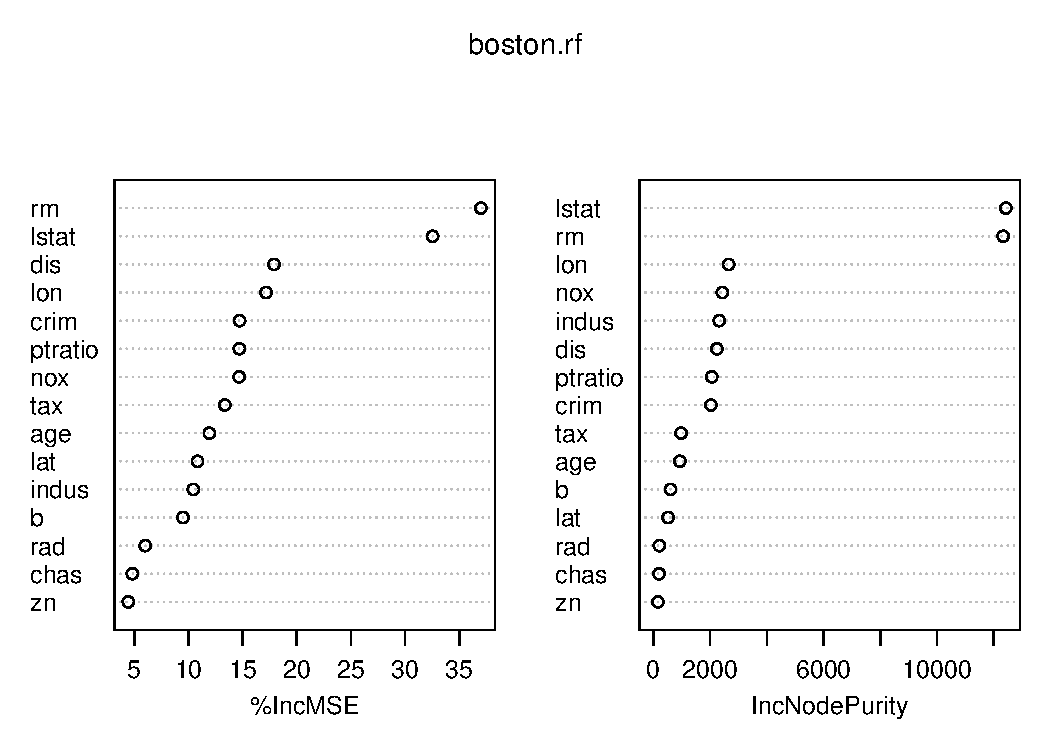
\includegraphics[width=1.0\linewidth]{boston_rf_vimp}
  \caption{Dotchart of variable importance scores for the Boston housing data based on a random forest with 500 trees.}
  \label{fig:plotmo_vs_partial}
\end{figure}


%%%%%%%%%%%%%%%%%%%%%%%%%%%%%%%%%%%%%%%%%%%%%%%%%%%%%%%%%%%%%%%%%%%%%%%%%%%%%%%%
% Single predictor PDPs
%%%%%%%%%%%%%%%%%%%%%%%%%%%%%%%%%%%%%%%%%%%%%%%%%%%%%%%%%%%%%%%%%%%%%%%%%%%%%%%%
\subsection{Single predictor PDPs}

As previously mentioned, the \code{randomForest} package has its own \code{partialPlot} function for visualizing the partial dependence of the response on a single predictor---the keywords here are "single predictor". For example, the following snippet of code plots the partial dependence of \code{cmedv} on \code{lstat}:
\begin{example}
partialPlot(boston.rf, pred.data = boston, x.var = "lstat")
\end{example}
The same plot can be achieved using the \code{partial} function and setting \code{plot = TRUE} (see the left side of Figure~\ref{fig:pd_lstat}):
\begin{example}
library(pdp)
partial(boston.rf, pred.var = "lstat", plot = TRUE)
\end{example}
The only difference is that \pkg{pdp} uses the \pkg{lattice} graphics package to produce all of its displays.

For a more customizable plot, we can set \code{plot = FALSE} in the call to \code{partial} and then use the \code{plotPartial} function on the resulting data frame. This is illustrated in the example below which increases the line width, adds a LOESS smooth, and customizes the $y$-axis label. The result is displayed in the right side of Figure~\ref{fig:pd_lstat}. \strong{Note:} to encourage writing more readable code, the \dfn{pipe} operator \code{\%>\%} provided by the \CRANpkg{magrittr} package \citep{magrittr-pkg} is exported whenever \pkg{pdp} is loaded.
\begin{example}
boston.rf %>%  # the %>% operator is read as "and then"
  partial(pred.var = "lstat") %>%
  plotPartial(smooth = TRUE, lwd = 2, ylab = expression(f(lstat)))
\end{example}

\begin{figure}[!htbp]
  \centering
  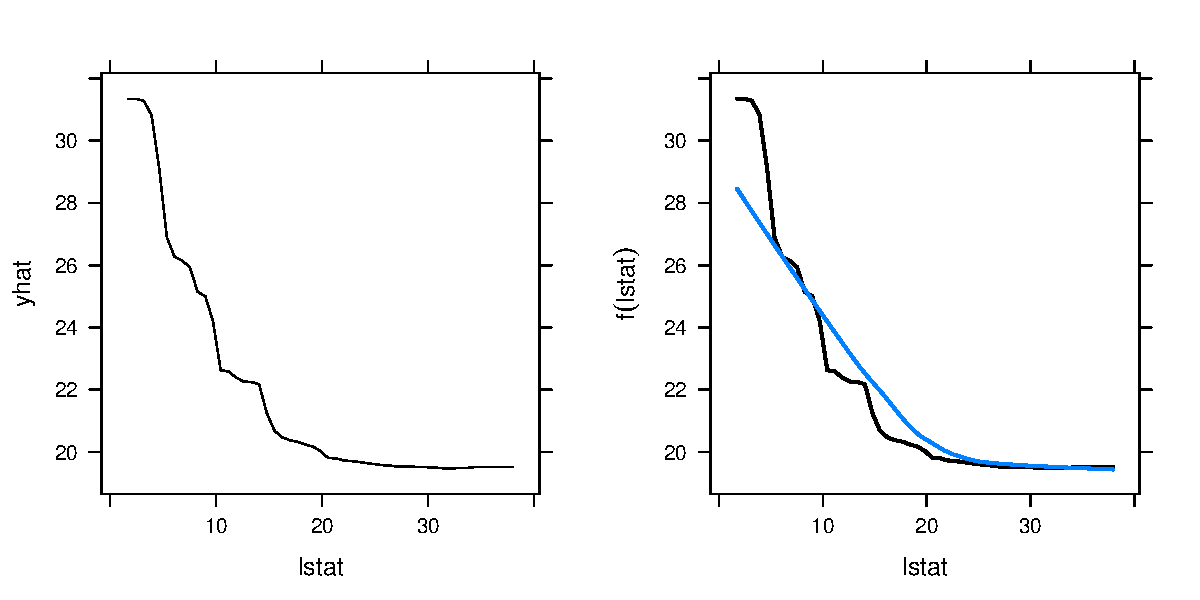
\includegraphics[width=1.0\linewidth]{pd_lstat}
  \caption{Partial dependence of \code{cmedv} on \code{lstat} based on a random forest. \textit{Left}: Default plot. \textit{Right}: Customized plot obtained using the \code{plotPartial} function.}
  \label{fig:pd_lstat}
\end{figure}


%%%%%%%%%%%%%%%%%%%%%%%%%%%%%%%%%%%%%%%%%%%%%%%%%%%%%%%%%%%%%%%%%%%%%%%%%%%%%%%%
% Multi-predictor PDPs
%%%%%%%%%%%%%%%%%%%%%%%%%%%%%%%%%%%%%%%%%%%%%%%%%%%%%%%%%%%%%%%%%%%%%%%%%%%%%%%%
\subsection{Multi-predictor PDPs}

The benefit of using \code{partial} is threefold: (1) it is a generic function that can be used for various types of fitted models (not just random forests), (2) it will allow for any number of predictors to be used (e.g., multivariate displays), and (3) it can utilize any of the parallel backends supported by the \CRANpkg{foreach} package \citep{foreach-pkg}; we discuss parallel execution in a later section. For example, the following code chunk uses the random forest model to assess the joint effect of \code{lstat} and \code{rm} on \code{cmedv}. The results, which make use of various \code{plotPartial} options, are displayed in Figure~\ref{fig:pd_lstat_rm}.
\begin{example}
rwb <- colorRampPalette(c("red", "white", "blue"))
pd <- partial(boston.rf, pred.var = c("lstat", "rm"))
plotPartial(pd)
plotPartial(pd, contour = TRUE, col.regions = rwb)
plotPartial(pd, levelplot = FALSE, zlab = "cmedv", drape = TRUE,
            colorkey = TRUE, screen = list(z = -20, x = -60))
\end{example}
\strong{Note:} the default color map for level plots is the color blind-friendly matplotlib \citep{hunter-matplotlib-2007} 'viridis' color map provided by the \CRANpkg{viridis} package \citep{viridis-pkg}.

\begin{widefigure}[htbp]
  \centering
  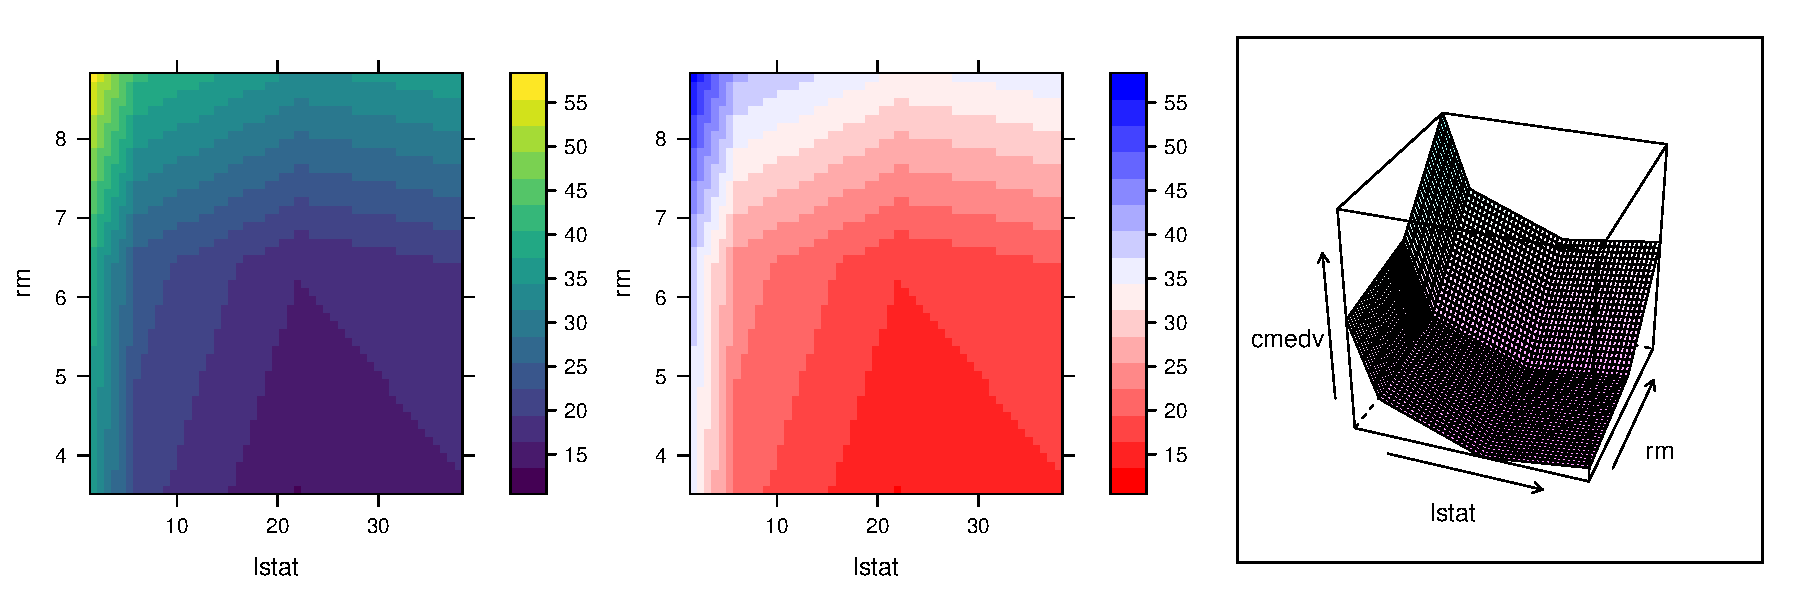
\includegraphics[width=1.0\linewidth]{pd_lstat_rm}
  \caption{Partial dependence of \code{cmedv} on \code{lstat} and \code{rm} based on a random forest. \textit{Left}: Default plot. \textit{Middle}: With contour lines and a different color palette. \textit{Right}: Using a 3-D surface.}
  \label{fig:pd_lstat_rm}
\end{widefigure}


%%%%%%%%%%%%%%%%%%%%%%%%%%%%%%%%%%%%%%%%%%%%%%%%%%%%%%%%%%%%%%%%%%%%%%%%%%%%%%%%
% Avoiding extrapolation
%%%%%%%%%%%%%%%%%%%%%%%%%%%%%%%%%%%%%%%%%%%%%%%%%%%%%%%%%%%%%%%%%%%%%%%%%%%%%%%%
\subsection{Avoiding extrapolation}

It is not wise to draw conclusions from PDPs in regions outside the area of the training data. Here we describe two ways to mitigate the risk of extrapolation in PDPs: rug displays and convex hulls. Rug displays are one-dimensional plots added to the axes. Both \code{partial} and \code{plotPartial} have a \code{rug} option that, when set to \code{TRUE}, will display the deciles of the distribution (as well as the minimum and maximum values) for the predictors on the horizontal and vertical axes. The following snippet of code produces the left display in Figure~\ref{fig:partial_extrap}.
\begin{example}
partial(boston.rf, pred.var = "lstat", plot = TRUE, rug = TRUE)
\end{example}

In two or more dimensions, plotting the convex hull is more informative; it outlines the region of the predictor space that the model was trained on. When \code{chull = TRUE}, the convex hull of the first two dimensions of $\boldsymbol{z}_s$ (i.e., the first two variables supplied to \code{pred.var}) is computed; for example, if you set \code{chull = TRUE} in the call to \code{partial} only the region within the convex hull of the first two variables is plotted. Over interpreting the PDP outside of this region is considered extrapolation and is ill-advised. The right display in Figure~\ref{fig:partial_extrap} was produced using:
\begin{example}
partial(boston.rf, pred.var = c("lstat", "rm"), plot = TRUE, chull = TRUE)
\end{example}

\begin{figure}[!htbp]
  \centering
  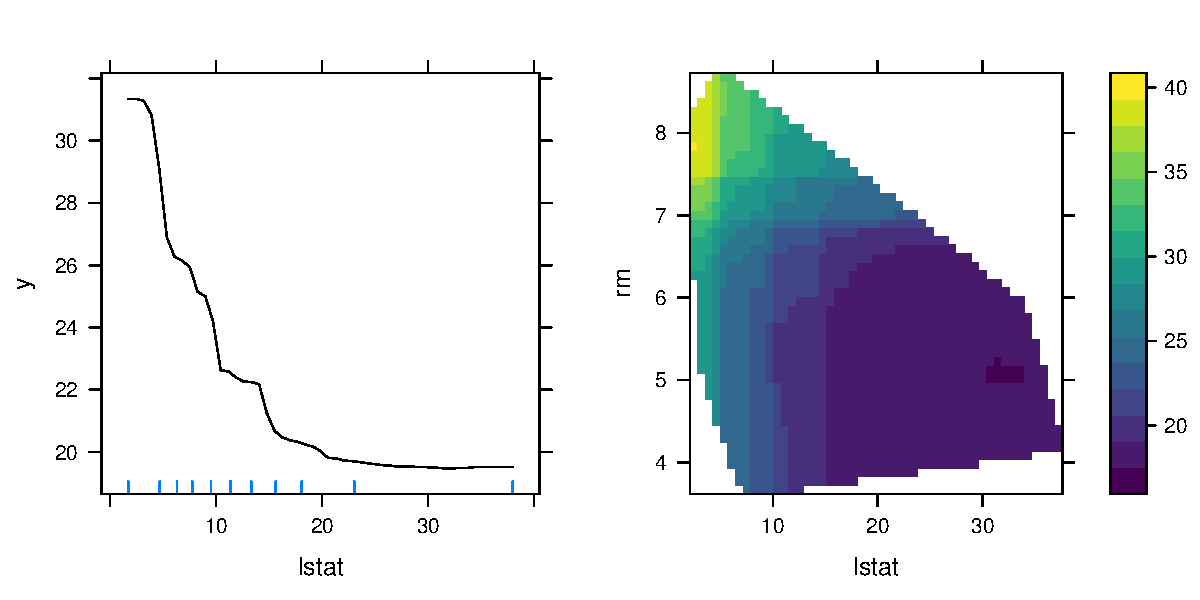
\includegraphics[width=1.0\linewidth]{partial_extrap}
  \caption{Examples of PDPs with the addition of a rug display (left) and a convex hull (right).}
  \label{fig:partial_extrap}
\end{figure}


%%%%%%%%%%%%%%%%%%%%%%%%%%%%%%%%%%%%%%%%%%%%%%%%%%%%%%%%%%%%%%%%%%%%%%%%%%%%%%%%
% Addressing computational concerns
%%%%%%%%%%%%%%%%%%%%%%%%%%%%%%%%%%%%%%%%%%%%%%%%%%%%%%%%%%%%%%%%%%%%%%%%%%%%%%%%
\subsection{Addressing computational concerns}

Constructing PDPs can be quite computationally expensive. Several strategies are available to ease the computational burden in larger problems. For example, there is no need to compute partial dependence of \code{cmedv} using each unique value of \code{rm} in the training data (which would require $k = 446$ passes over the data!). We could get very reasonable results using a reduced number of points. Current options are to use a grid of equally spaced values in the range of the variable of interest; the number of points can be controlled using the \code{grid.resolution} option in the call to \code{partial}. Alternatively, a user-specified grid of values (e.g., containing specific quantiles of interest) can be supplied through the \code{pred.grid} argument. To demonstrate, the following snippet of code computes the partial dependence of \code{cmedv} on \code{rm} using each option; the results are displayed in Figure~\ref{fig:partial_manual}.
\begin{example}
partial(boston.rf, "rm", plot = TRUE)
partial(boston.rf, "rm", grid.resolution = 30, plot = TRUE)
partial(boston.rf, "rm", pred.grid = data.frame(rm = 3:9), plot = TRUE)
\end{example}

\begin{widefigure}[htbp]
  \centering
  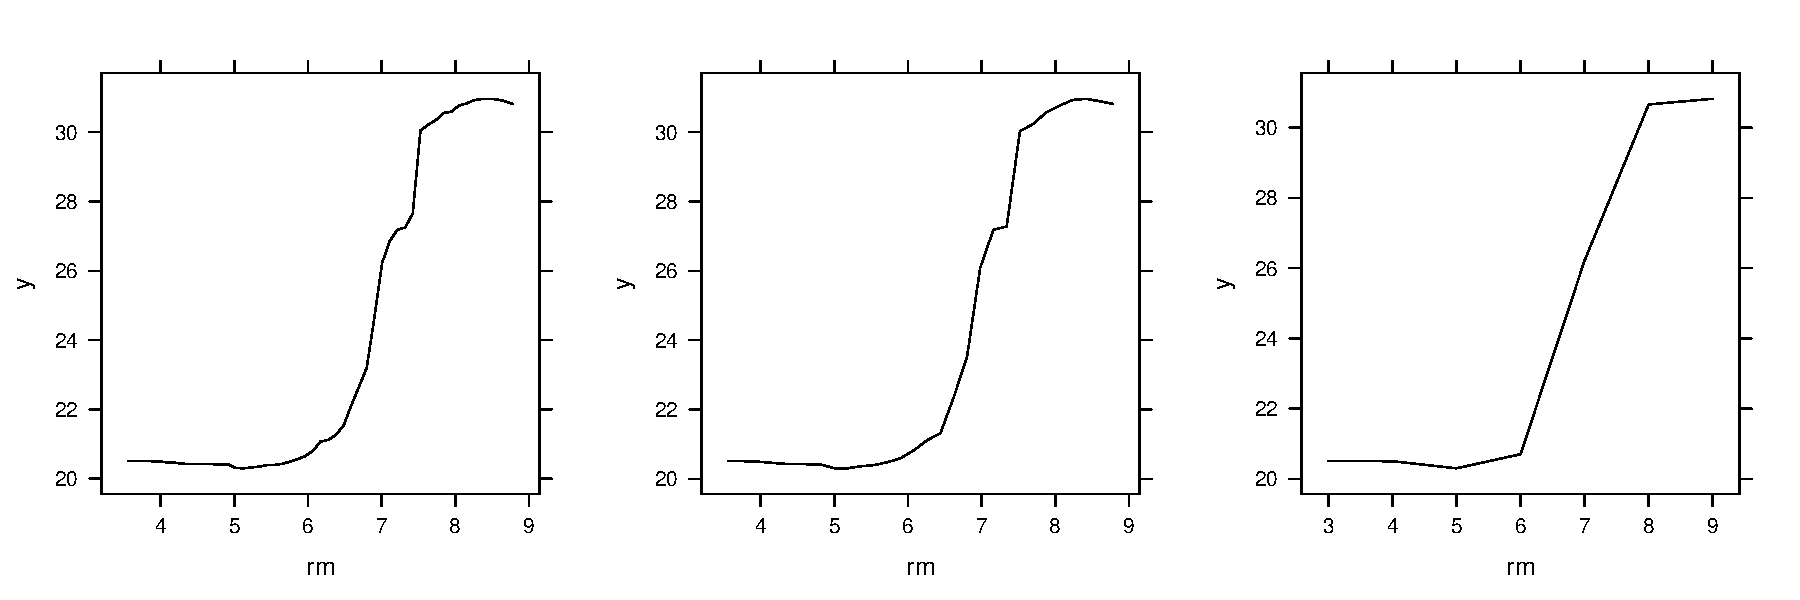
\includegraphics[width=0.8\linewidth]{partial_manual}
  \caption{Partial dependence of \code{cmedv} on \code{rm}. \textit{Left}: Default plot. \textit{Middle}: Using a reduced grid size. \textit{Right}: Using a user-specified grid.}
  \label{fig:partial_manual}
\end{widefigure}

The \code{partial} function relies on the \CRANpkg{plyr} package \citep{plyr-pkg}, rather than R's built-in \code{for} loops. This makes it easy to request progress bars (e.g., \code{progress = "text"}) or run \code{partial} in parallel. In fact, \code{partial} can use any of the parallel backends supported by the \pkg{foreach} package. To use this functionality, we must first load and register a supported parallel backend [e.g., \CRANpkg{doMC} \citep{doMC-pkg} or \CRANpkg{doParallel} \citep{doParallel-pkg}].

To illustrate, we will use the Los Angeles ozone pollution data described in \citet{breiman-1985-estimating}. The data contain daily measurements of ozone concentration (\code{ozone}) along with eight meteorological quantities for 330 days in the Los Angeles basin in 1976. The data are available from \url{http://statweb.stanford.edu/~tibs/ElemStatLearn/datasets/LAozone.data}. Details, including variable information, are available from \url{http://statweb.stanford.edu/~tibs/ElemStatLearn/datasets/LAozone.info}. The following code chunk loads the data into R:
\begin{example}
ozone <- read.csv(paste0("http://statweb.stanford.edu/~tibs/ElemStatLearn/",
                         "datasets/LAozone.data"), header = TRUE)
\end{example}

Next, we use the multivariate adaptive regression splines (MARS) algorithm introduced in \citet{friedman-1991-mars} to model ozone concentration as a nonlinear function of the eight meteorological variables plus day of the year; we allow for up to three-way interactions.
\begin{example}
ozone.mars <- earth(ozone ~ ., data = ozone, degree = 3)
summary(ozone.mars)
\end{example}
The MARS model produced a generalized $R^2$ of $0.79$, similar to what was reported in \citet{breiman-1985-estimating}. A single three-way interaction was found involving the predictors
\begin{itemize}
  \item \code{wind}: wind speed (mph) at Los Angeles International Airport (LAX)
  \item \code{temp}: temperature ($^oF$) at Sandburg Air Force Base
  \item \code{dpg}: the pressure gradient (mm Hg) from LAX to Dagget, CA
\end{itemize}
To understand this interaction, we can use a PDP. However, since the partial dependence between three continuous variables can be computationally expensive, we will run \code{partial} in parallel.

Setting up a parallel backend is rather straightforward. To demonstrate, the following snippet of code sets up the \code{partial} function to run in parallel on Unix-like systems\footnote{This example will not run on Windows.} using the \pkg{doParallel} package.
\begin{example}
library(doParallel)  # load parallel backend
registerDoParallel(cores = 4)  # use 4 cores
\end{example}
Now, to run \code{partial} in parallel, all we have to do is invoke the \code{parallel = TRUE} option and the rest is taken care of by the internal call to \pkg{plyr} and the parallel backend we loaded. This is illustrated in the code chunk below which obtains the partial dependence of \code{ozone} on \code{wind}, \code{temp}, and \code{dpg} in parallel. The result is displayed in Figure~\ref{fig:partial_par}.
\begin{example}
partial(ozone.mars, pred.var = c("wind", "temp", "dpg"), plot = TRUE,
        chull = TRUE, parallel = TRUE)
\end{example}

\begin{figure}[!htbp]
  \centering
  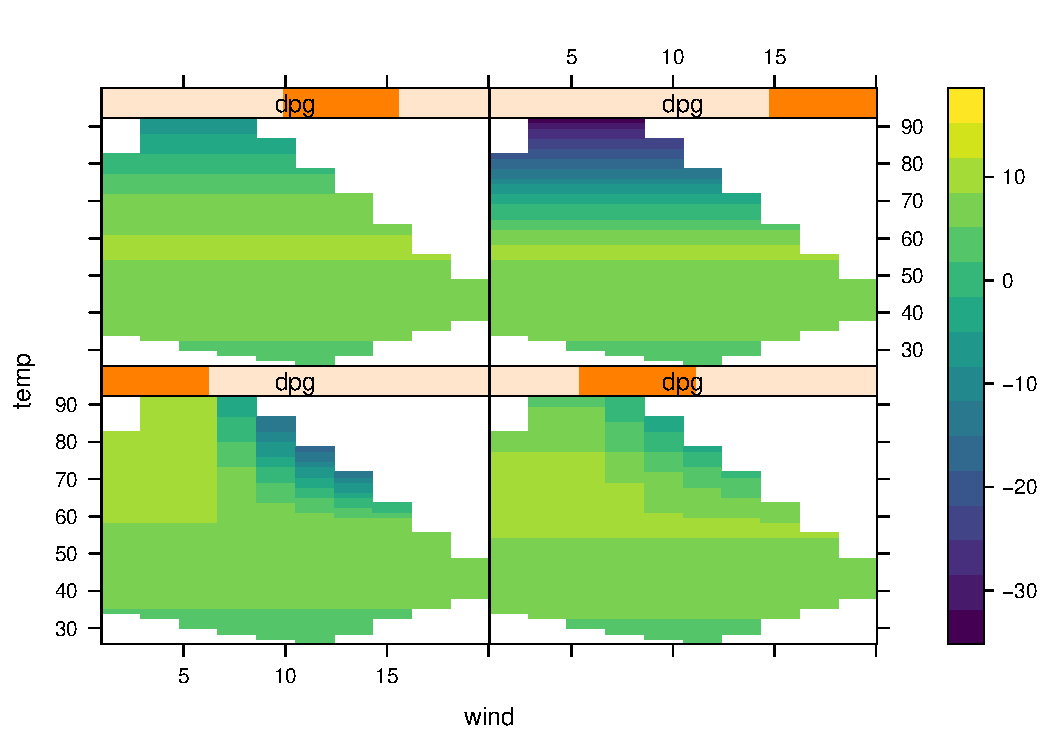
\includegraphics[width=0.8\linewidth]{partial_par}
  \caption{Partial dependence of \code{ozone} on \code{wind}, \code{temp}, and \code{dpg}. Since \code{dpg} is contiuous, it is first converted to a shingle; in this case, four groups with 10\% overlap.}
  \label{fig:partial_par}
\end{figure}

It is important to note that when using more than two predictor variables, \code{plotPartial} produces a trellis display. The first two variables given to \code{pred.var} are used for the horizontal and vertical axes, and additional variables define the panels. If the panel variables are continuous, then shingles\footnote{A shingle is a special Trellis data structure that consists of a numeric vector along with intervals that define the "levels" of the shingle. The intervals may be allowed to overlap.} are produced first using the equal count algorithm (see, for example, \code{?lattice::equal.count}). Hence, it will be more effective to use categorical variables to define the panels in higher dimensional displays when possible.


\subsection{Classification problems}

For classification problems, partial dependence functions are on a scale similar to the logit; see, for example, \citet[pp. 369---370]{hastie-elements-2009}. Suppose the response is categorical with $K$ levels, then for each class we compute
\begin{equation}
\label{eqn:avg-logit}
f_k(x) = \log\left[p_k(x)\right] - \frac{1}{K}\sum_{i = 1}^K\log\left[p_k(x)\right], \quad k = 1, 2, \dots, K,
\end{equation}
where $p_k(x)$ is the predicted probability for the $k$-th class. Plotting $f_k(x)$ helps us understand how the log-odds for the $k$-th class depends on different subsets of the predictor variables.

To illustrate, we consider Edgar Anderson's iris data from the \pkg{datasets} package. The \code{iris} data frame contains the sepal length, sepal width, petal length, and petal width (in centimeters) for 50 flowers from each of three species of iris:  setosa, versicolor, and virginica. We fit a support vector machine with a Gaussian radial basis function kernel to the data using the \code{svm} function in the \pkg{e1071} package (the tuning parameters were determined using 5-fold cross-validation).
\begin{example}
library(e1071)
iris.svm <- svm(Species ~ ., data = iris, kernel = "radial", gamma = 0.75,
                cost = 0.25, probability = TRUE)
\end{example}
\strong{Note:} the \code{partial} function has to be able to extract the predicted probabilities for each class, so it is necessary to set \code{probability = TRUE} in the call to \code{svm}.

Next, we plot the partial dependence of \code{Species} on both \code{Petal.Width} and \code{Petal.Length} for each of the three classes. The result is displayed in Figure~\ref{fig:partial_iris}. %Note that we had to supply the original training data to \code{partial} through the \code{train} option. This is necessary for fitted model objects that don't store a copy of the training data (e.g., model fitting functions that don't rely on a formula method).
\begin{example}
pd <- NULL
for (i in 1:3) {
  tmp <- partial(iris.svm, pred.var = c("Petal.Width", "Petal.Length"),
                 which.class = i, grid.resolution = 101, progress = "text")
  pd <- rbind(pd, cbind(tmp, Species = levels(iris$Species)[i]))
}

library(ggplot2)
ggplot(pd, aes(x = Petal.Width, y = Petal.Length, z = y, fill = y)) +
  geom_tile() +
  geom_contour(color = "white", alpha = 0.5) +
  scale_fill_distiller(name = "Average\nlogit", palette = "Spectral") +
  theme_bw() +
  facet_grid(~ Species)
\end{example}

\begin{figure}[!htbp]
  \centering
  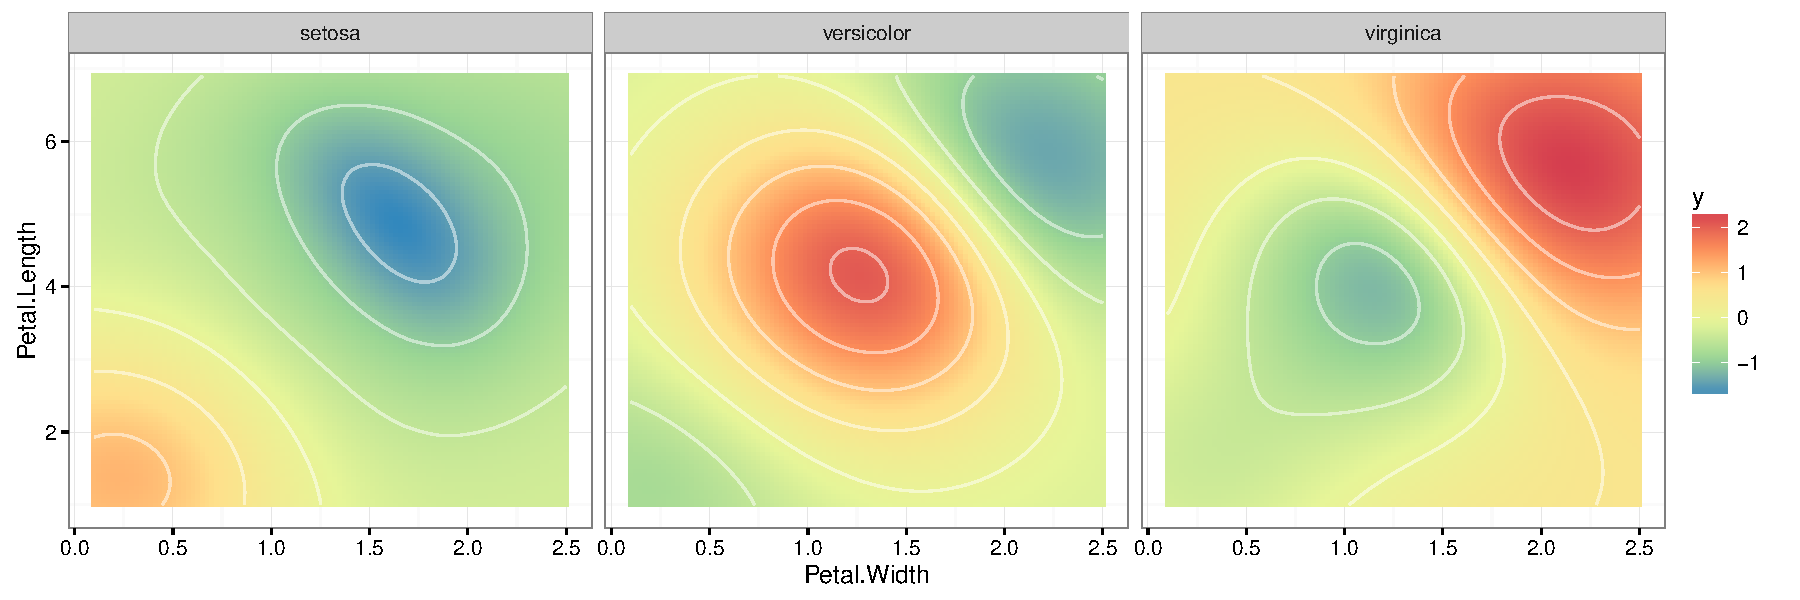
\includegraphics[width=1.0\linewidth]{partial_iris_svm}
  \caption{Partial dependence of species on petal width and petal length for the iris data.}
  \label{fig:partial_iris}
\end{figure}


%%%%%%%%%%%%%%%%%%%%%%%%%%%%%%%%%%%%%%%%%%%%%%%%%%%%%%%%%%%%%%%%%%%%%%%%%%%%%%%%
% Using partial with xgboost
%%%%%%%%%%%%%%%%%%%%%%%%%%%%%%%%%%%%%%%%%%%%%%%%%%%%%%%%%%%%%%%%%%%%%%%%%%%%%%%%
\subsection{Using partial with the XGBoost library}
\label{sec:xgboost}

To round out our discussion, we provide one last example using a recently popular (and successful!) machine learning tool. XGBoost, short for eXtreme Gradient Boosting, is a popular library providing optimized distributed gradient boosting that is specifically designed to be highly efficient, flexible and portable. The associated R package \pkg{xgboost} has been used to win a number of \href{https://www.kaggle.com/}{Kaggle competitions}. It has been shown to be many times faster than the well known \pkg{gbm} package. However, unlike \pkg{gbm}, \pkg{xgboost} does not have built-in functions for constructing PDPs. Fortunately, the \pkg{pdp} package can be used to fill this gap.

For illustration, we return to the Boston housing data. The code chunk below fits an \pkg{xgboost} model to the \code{boston} data frame from Section~\ref{sec:boston}; the tuning parameters were predetermined using 5-fold cross-validation. (Make sure you are using version 0.6-0 or later of \pkg{xgboost}: \url{https://github.com/dmlc/xgboost/tree/master/R-package}.)
\begin{example}
set.seed(102)  # for reproducibility
boston.xgb <- xgboost(data = data.matrix(subset(boston, select = -cmedv)),
                      label = boston$cmedv, objective = "reg:linear",
                      nrounds = 2000, max_depth = 3, eta = 0.01)
\end{example}

To use \code{partial} with the \code{"xgb.Booster"} class, we need to supply the original training data (minus the response) in the call to \code{partial}. The following snippet of code computes the partial dependence of \code{cmedv} on both \code{rm} and \code{lstat}, individually and together. The results are displayed in Figure~\ref{fig:boston_xgb}. \strong{Note:} while \code{xgboost} requires the training data to be an object of class \code{"matrix"}, \code{"dgCMatrix"}, or \code{"xgb.DMatrix"}, \code{partial} requires a \code{"data.frame"}.
\begin{example}
pred.list <- list("lstat", "rm", c("lstat", "rm"))
for (x in pred.list) {
  partial(boston.xgb, pred.var = x, plot = TRUE, smooth = TRUE, rug = TRUE,
          chull = TRUE, train = subset(boston, select = -cmedv))
}
\end{example}

\begin{figure}[!htbp]
  \centering
  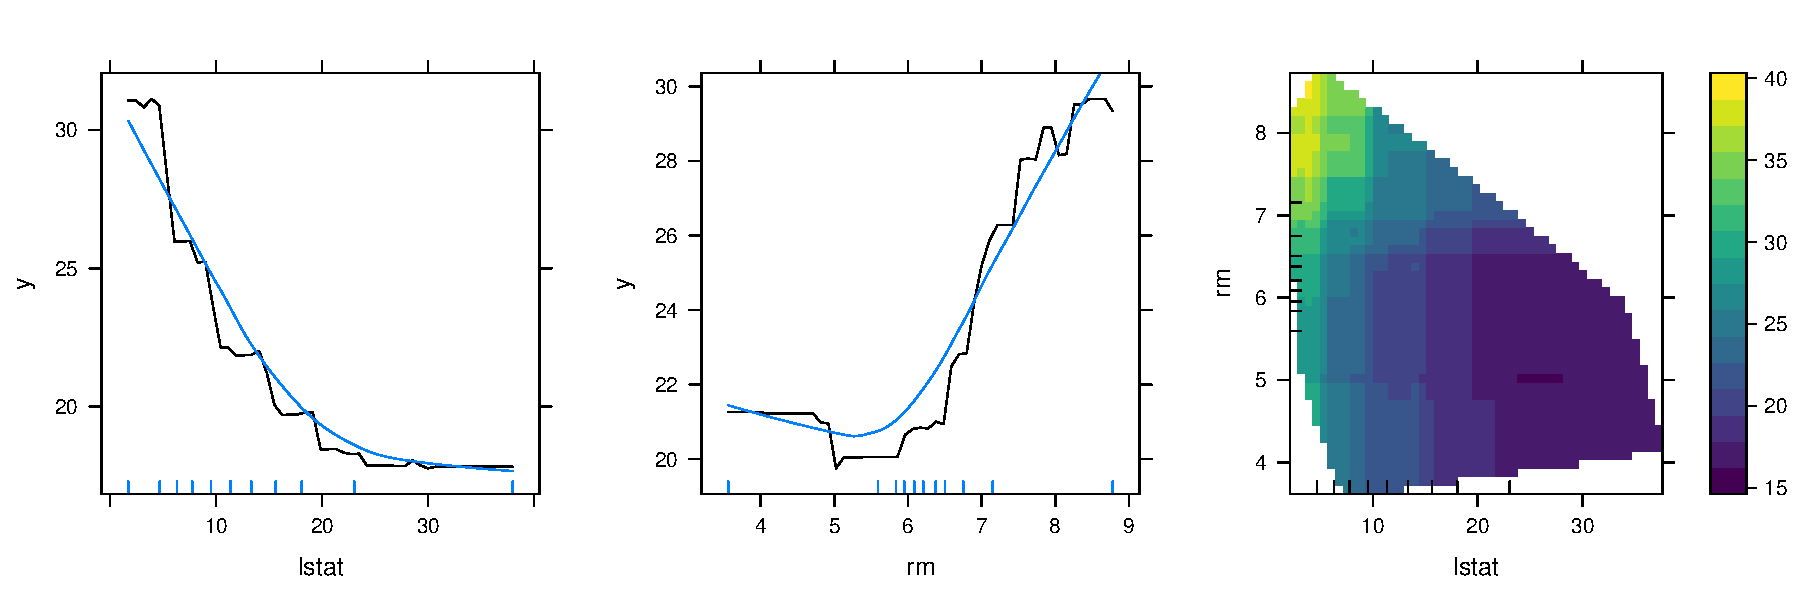
\includegraphics[width=1.0\linewidth]{boston_xgb}
  \caption{PDPs for the top two most important variables in the Boston housing data using XGBoost. Compare this to the random forest results displayed in Figures~\ref{fig:partial_extrap}-\ref{fig:partial_manual}.}
  \label{fig:boston_xgb}
\end{figure}


%%%%%%%%%%%%%%%%%%%%%%%%%%%%%%%%%%%%%%%%%%%%%%%%%%%%%%%%%%%%%%%%%%%%%%%%%%%%%%%%
% Using partial with caret
%%%%%%%%%%%%%%%%%%%%%%%%%%%%%%%%%%%%%%%%%%%%%%%%%%%%%%%%%%%%%%%%%%%%%%%%%%%%%%%%


%%%%%%%%%%%%%%%%%%%%%%%%%%%%%%%%%%%%%%%%%%%%%%%%%%%%%%%%%%%%%%%%%%%%%%%%%%%%%%%%
% Summary
%%%%%%%%%%%%%%%%%%%%%%%%%%%%%%%%%%%%%%%%%%%%%%%%%%%%%%%%%%%%%%%%%%%%%%%%%%%%%%%%
\section{Summary}

PDPs can be used to graphically examine the dependence of the response on low cardinality subsets of the features, accounting for the average effect of the other predictors. In this paper, we showed how to construct PDPs for various types of black box models in R using the \pkg{pdp} package. We also briefly discussed related approaches available in other R packages. Suggestions to avoid extrapolation and high execution times were discussed and demonstrated via examples.

In terms of future development, \pkg{pdp} can be expanded in a number of ways. For example, it would be useful to have the ability to construct PDPs for black box survival models---like conditional random forests with censored response. It would also be worthwhile to implement the partial dependence-based $H$-statistic \citep{friedman-2008-predictive} for assessing the strength of interaction between predictors.


%%%%%%%%%%%%%%%%%%%%%%%%%%%%%%%%%%%%%%%%%%%%%%%%%%%%%%%%%%%%%%%%%%%%%%%%%%%%%%%%
% Summary
%%%%%%%%%%%%%%%%%%%%%%%%%%%%%%%%%%%%%%%%%%%%%%%%%%%%%%%%%%%%%%%%%%%%%%%%%%%%%%%%
\section{Acknowledgments}

TBD.


%%%%%%%%%%%%%%%%%%%%%%%%%%%%%%%%%%%%%%%%%%%%%%%%%%%%%%%%%%%%%%%%%%%%%%%%%%%%%%%%
% Back matter
%%%%%%%%%%%%%%%%%%%%%%%%%%%%%%%%%%%%%%%%%%%%%%%%%%%%%%%%%%%%%%%%%%%%%%%%%%%%%%%%

\bibliography{greenwell}

\address{Brandon M. Greenwell\\
  Infoscitex Corporation\\
  4027 Colonel Glenn Highway\\
  Suite 210\\
  Dayton, OH 45431-1672\\
  United States of America\\}
\email{greenwell.brandon@gmail.com}
